\documentclass[titlepage]{article}

\usepackage{tipa}
\usepackage{titlepic}
\usepackage{graphicx}
\usepackage{hyperref}
\usepackage{xcolor}
\usepackage{float}
\usepackage{minted}
\usepackage[export]{adjustbox}

\DeclareGraphicsExtensions{.pdf,.png,.jpg}

\definecolor{linkcol}{RGB}{50,50,50}
\hypersetup{
    colorlinks=true,
    linkcolor=linkcol
}


\title{
\includegraphics[width=200pt, height=260pt]{../../images/trdrop_logo_text.eps} \\[50pt]
T(ea)rdrop - a video analysis software}
\author{Alexander Isenko\\Mujo Alic}
\date{}

\begin{document}

\maketitle

\newpage

\section{Abstract}
Offline feature extraction from streams in a single pass with automatic parallelization is a useful structure for several applications. We showcase our interpretation of this concept on a video analysis software by creating a type based parallelization with a transformation pipeline and external coupling. This allows a race-conditions-free, comprehensible interface to add features without depending on previous tasks while maintaining a sound performance.

\section{Introduction}

\textbf{trdrop} - pronounced [\textit{\textipa{'te@(r),drAp}}]. \\[2mm]
\hfill
The gamer of today wants to buy the best hardware to get his money's worth. One of the console benchmarks is to run games at least as smooth as their competitors. To test this without bias, one needs to capture the raw video stream and perform several calculations on the uncompressed video to detect framedrops and tears. We present a configurable command line tool to analyze multiple big, raw videos in parallel, insert a visual representation for the outcoming data and encode the videos in a single pass. 

\section{Features}

The following features are included in \textbf{v0.1}:

\begin{itemize}
    \item determine the real fps of the incoming video files with a sliding window of the capture rate
    \item show the fps as text in the video
    \item export the resulting video into a youtube friendly format (\href{https://support.google.com/youtube/answer/1722171}{google-terms})
    \item create a csv-log with the framerate and every tear + fps
    \item visualize the fps in a plot
    \item import up to 2 \texttt{.raw} video files with a size of (0 - 15) \texttt{GB}
        \item analyze the videos in parallel
    
\end{itemize}

\section{Program Diagram}

\begin{figure}[H]
\hspace{-20mm}
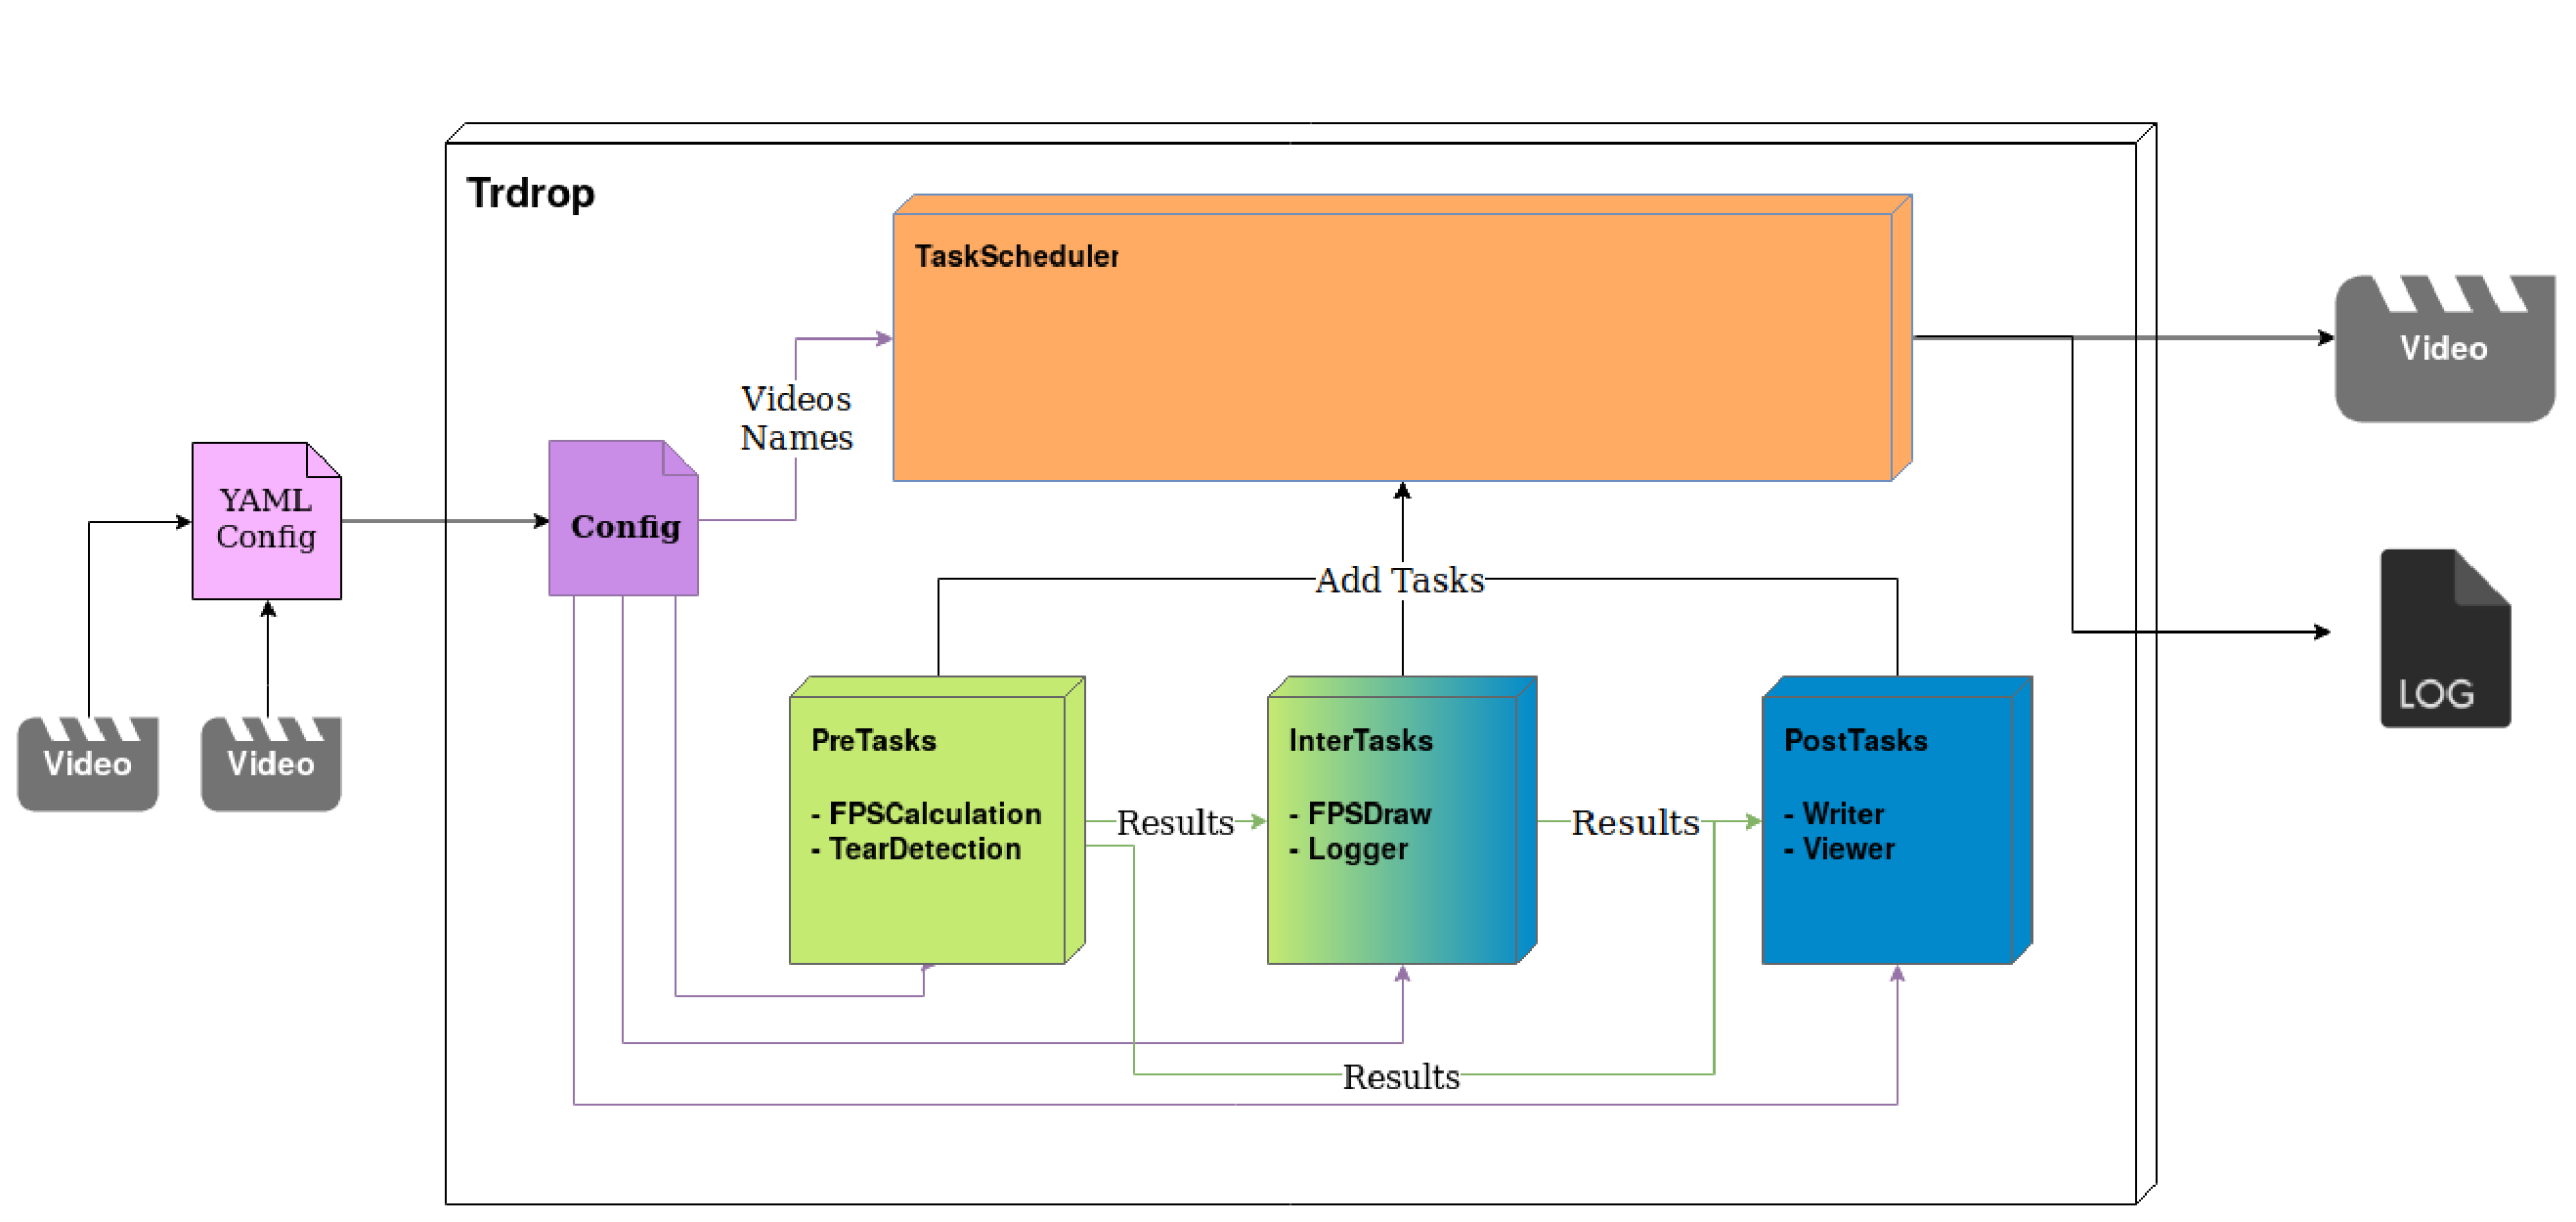
\includegraphics[width=430pt,left]{../../images/trdrop-main-system.eps}
\caption{Main system diagram}
\label{fig:main-system}
\end{figure}

The program has three main concepts:

\begin{description}
    \item [Config sanitizing] - rest of the programs deals with data in a valid state
    \item [Tasks] - externally coupled separation of \textit{model} and \textit{view} for every algorithm allows for a parallelizable computation
    \item [TaskScheduler] - configurable pipeline which traverses the videofiles in a \\single pass and applies tasks in parallel to it
\end{description}

\subsection{Config}
The program is configurable through a \textit{YAML} file as seen in Fig.\ref{fig:main-system}, where you can customize the fps calculation, like the fps-refresh rate, fps precision and other options. The \textit{Config} parses this file, checks the inputs for sanity and forwards it to the internal logic. The forwarding is implemented with \textbf{control coupling}. \\

\begin{figure}[H]
\begin{minted}[linenos]{c++}
using pretask = std::function<void(const cv::Mat & prev
                                 , const cv::Mat & cur
                                 , const size_t currentFrame
                                 , const size_t videoIndex)>;

using intertask = std::function<void(cv::Mat & res
                                   , const size_t currentFrame
                                   , const size_t videoIndex)>;

using posttask = std::function<void(cv::Mat & merged
                                  , const size_t currentFrame)>;
\end{minted}
\caption{Interface definition of the three tasks}
\label{code:task-interfaces}
\end{figure}

\subsection{Tasks}
\label{header:tasks}

This proposed division of an algorithm into tasks in Fig.\ref{code:task-interfaces} demands a logical separation for the calculation and modification of the resulting video. It allows for an automatic parallelization of the calculations because of the external coupling down the pipeline. The tasks are divided in three kinds, which support the source-sink concept. They are added to the \textit{TaskScheduler} which runs them with the respective arguments in the order determined by their type.

\subsubsection{PreTask}
The \textit{pretask} described  takes two videoframes to use for calculations,
the current frame index and video index which activates the respective configuration of the task. This task has no access to modify the incoming stream of data, but may use external coupling to transmit calculation results down the pipeline. This fullfills the concept of a \textbf{source}.

\subsubsection{InterTask}
The \textit{intertask} defines the intermediate task, which has the access to modify the videoframe for each video seperately with their respective configuration. It may use information from \textit{pretasks} and modify the incoming datastream, but can also forward information to \textit{posttasks}. This fullfills the requirements of a \textbf{source} and \textbf{sink}.

\subsubsection{PostTask}
The \textit{posttask} gets access the merged datastream and can modify the resulting videoframe before it gets written to the disk. It may use all information passed down to it, but no previous task can be dependent on it's calculation. Therefore this is task is defined as a \textbf{sink}.

\newpage

\subsection{TaskScheduler}
\label{header:task-scheduler}

After the creation and coupling of the tasks, the \textit{TaskScheduler} implements the single pass pipeline in Fig.\ref{fig:source-sink}.

\begin{figure}[H]
\hspace{-30mm}
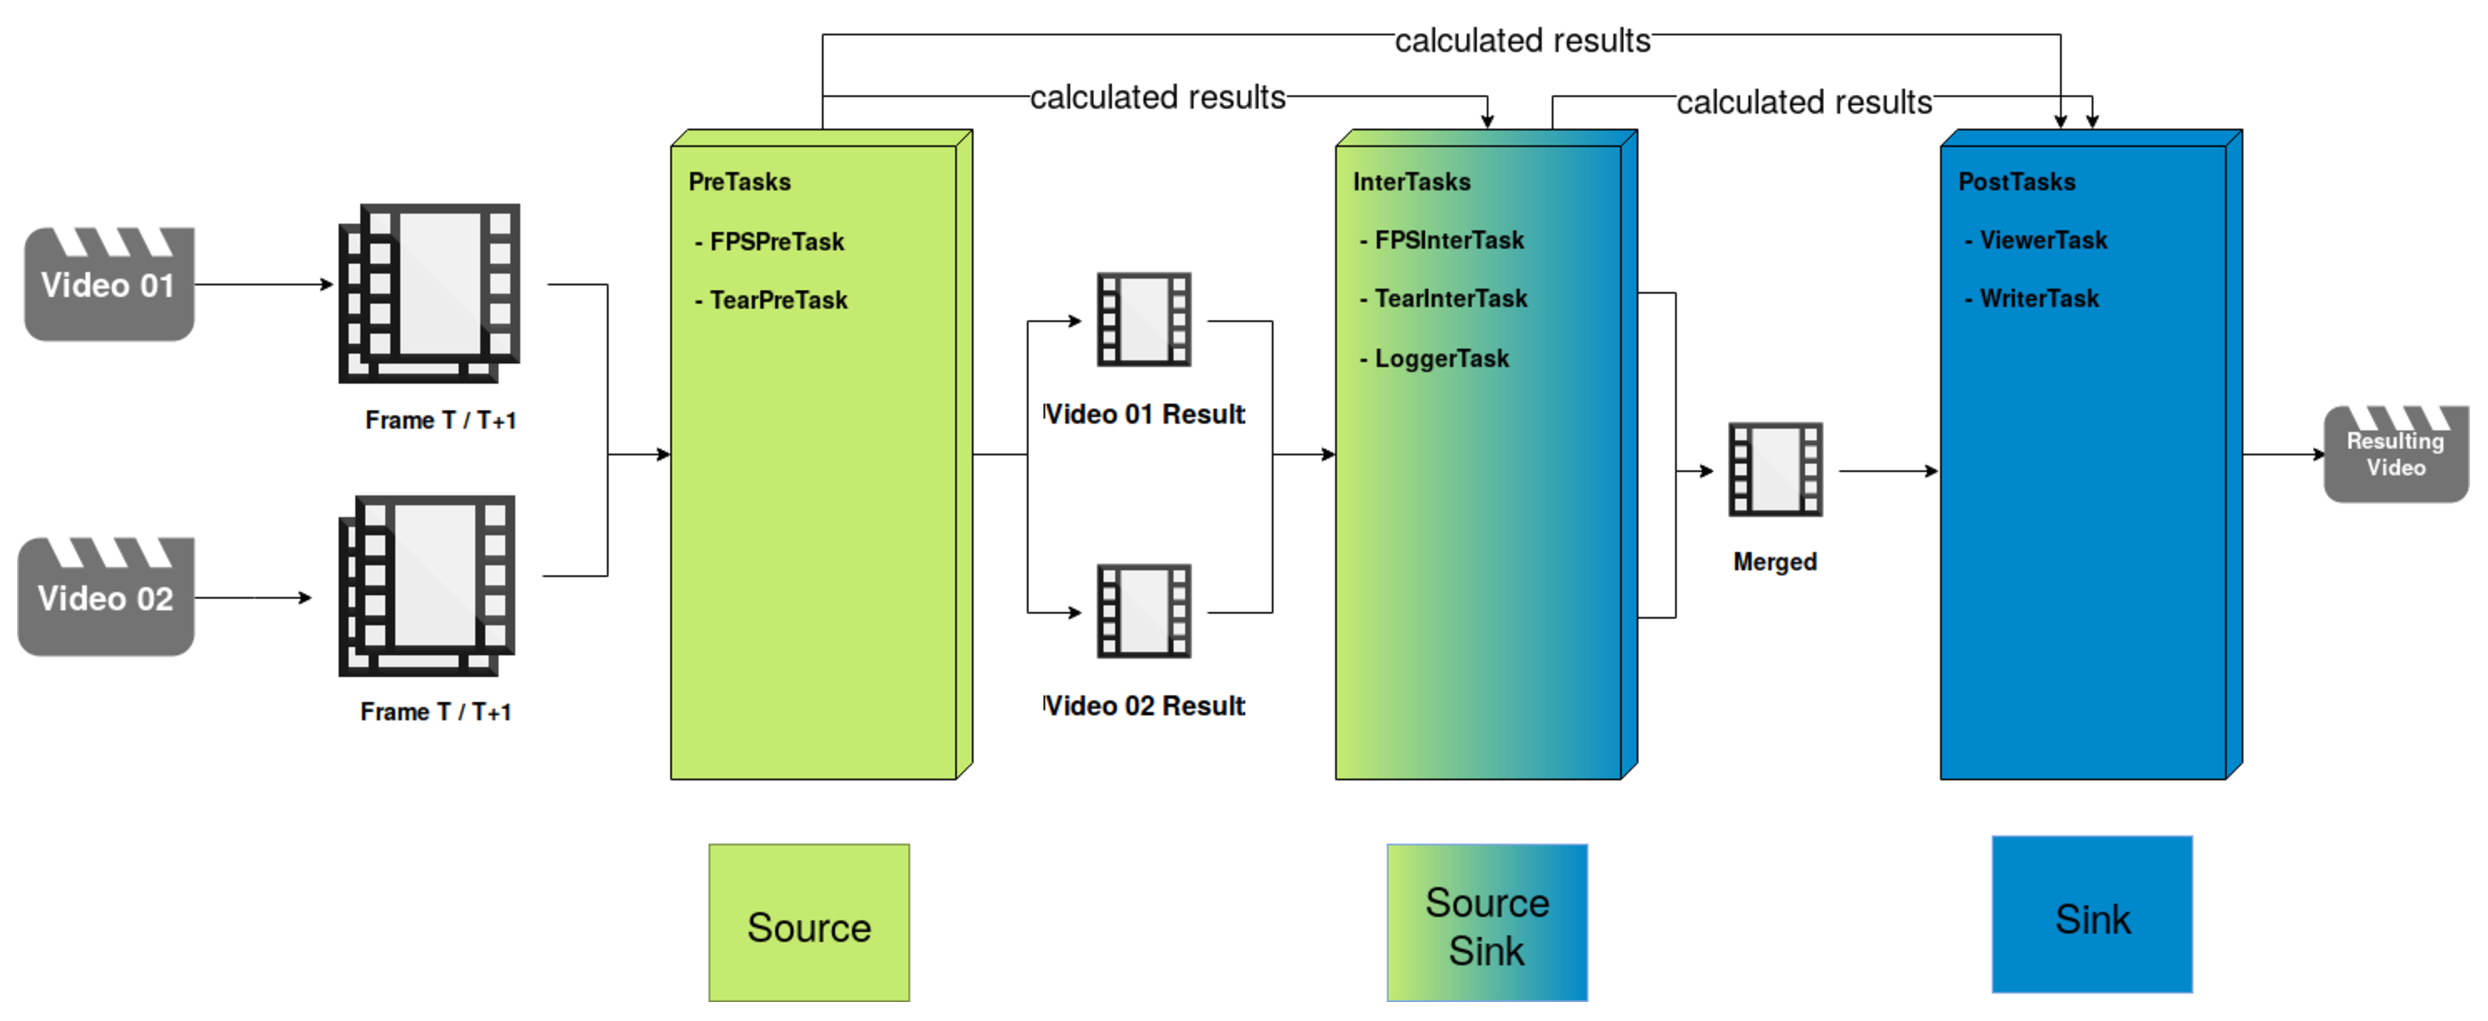
\includegraphics[width=500pt,left]{../../images/trdrop-source-sink.eps}
\caption{Task Pipeline}
\label{fig:source-sink}
\end{figure}
\hfill \\
It has always ``videos times 2'' frames in memory and forwards them to the \textit{pretasks} in parallel. The frame to modify is always at time \texttt{T}, because it will not be necessary for the next round of calculations.\\[4mm]
These will be passed to the \textit{intertasks} and modified accordingly. A single asynch call will be made for every video, but not for every \textit{intertask}, because these tasks are not commutative. \\[4mm]
The modified videoframes will be merged by the \textit{TaskScheduler} into one frame and transferred to the \textit{posttasks} which will be applied sequentially. \\
\hfill \\
After this round the frame at time \texttt{T + 1} will be the new frame \texttt{T'} and the next one will be loaded as \texttt{T' + 1}.
This loop aborts if any of the videos don't have any frames left.\\
\hfill \\
The intetion behind this scheduler was to abstract the looping through multiple videos and provide an interface where tasks can be defined without explicit iteration through frames.

\newpage
\section{Why not do it another way?}

In this paragraph we're going to stand up to some design decision and shortly explain why we took them.

\subsection{Callbacks vs. explicit Either data object\\ for task communication}

The idea behind the \texttt{Either} object were tasks that could fail, or not trigger because of certain events (e.g sleep for $n$ frames). Therefore a structure where we can call \texttt{successful()} was ideally suited. The choice for \texttt{Either} instead of \texttt{Maybe} was to be able to return an error value (e.g ``still calculating fps'').

\begin{figure}[H]
\begin{minted}[linenos]{c++}
if (fpsPreTask.result.successful()) {
    framerates = fpsPreT.result.getSuccess();
}
\end{minted}
\caption{Accessing the fpsPreTask calculation}
\label{code:fpspretask-glue}
\end{figure}
\hfill\\
Next to the explicit nature and descriptivity of this branch (Fig.\ref{code:fpspretask-glue}) in the main loop, we made the decision to make the \textit{tasks} responsible to store their results, so it would be possible to create a task without dependencies to the outer scope. Anybody who wants to get the result, can ask the task by themselves.\\
\hfill \\
In fact, we have an exceptional callback solution for the \textit{LoggerTask} (Fig.\ref{code:logger-init}), but this happend because we wanted to define to \texttt{string} representation of the logged values explicitly. These lambdas are not bound to the sources of the tasks and instead use the current value of the variable that stores the result. This way we don't have to check every time if the \textit{fpsPreTask} is successful, because the code in Fig.\ref{code:fpspretask-glue} updates it.

\begin{figure}[H]
\begin{minted}[linenos]{c++}
std::vector<function<std::string()>> convertions;
convertions.push_back([&]() {
  return string_format("%5i", scheduler.getCurrentFrameIndex());
});
convertions.push_back([&]() {
  return string_format("%6." + std::to_string(config.fpsPrecision) + "f", framerates);
});
LoggerTask<CSVFile> loggerT(config.logFile, 1, file, convertions);
\end{minted}
\caption{Creating the LoggerTask (shortened namespaces)}
\label{code:logger-init}
\end{figure}

\subsection{Automatic parallelization with DAGs}

Directed Acyclic Graphs are a very handy abstraction for complex dependency solving problems, but in our case we have the luxury to know that our computation is always linear, e.g we start with the first frame and end with last one. We also know that any computation has to run \textit{atmost} every timestep with an input of two frames (this may even be desired, even if the dependent result does not change).\\
\hfill \\
This domain specific knowledge allowed us to create the separation of three different tasks kinds which have different levels of parallelsim. If every computational result is initialized with a sane default value, we can define tasks that don't have any race conditions or wait times for unfinished calculations.\\
\hfill \\
It may be true that with DAGs we could be a little bit faster, because some \textit{intertasks} of \texttt{video01} may start before the \textit{pretasks} of \texttt{video02} are finished, but the real bottleneck is the encoding of the video in the desired codec. Instead of this little speedbump we have direct control over the way how the task behave and how often they are called.\\

\subsection{Do we really need three different tasks?}

The decision to use an interface for three tasks came gradually as we expected to work with only a \textit{pretask} and \textit{posttask} which already provides most of the advantages of in Chap.\ref{header:tasks}. The modification of the multiple videos in a non-sequential manner urged us to introduce the \textit{intertask}, which allows partial parallelization between different videos.\\
\hfill\\
Because of the externally coupled interface we provided, we expect to cover most of the future task and may introduce the \textbf{source} concept to the \textit{posttask} as well as the \textbf{sink} concept to the \textit{pretask}, if it seems fit. 

\end{document}

 